\documentclass[11pt]{article}
\usepackage{setspace} \singlespacing
\usepackage{graphicx} % Required for inserting images
\usepackage{fullpage}
\usepackage{amsmath}
\usepackage{url}
\setlength{\parindent}{0pt}


\title{Stroke Prediction Final Report}
\author{Kaushal Marimuthu, James Xu, Matthew Craig, Zixuan Weng}
\date{March 14, 2024}

\begin{document}

\maketitle

\section*{Outline}
Stroke is one of the leading causes of death in the United States. This project sets out to develop a comprehensive machine learning model capable of predicting stroke risk based on a variety of factors, including demographics, health conditions, and social status. Using a Kaggle dataset with over 5000 observations across 11 clinical trials; this paper aims to discover the complex interplay factors including gender, age, history of hypertension, heart disease, marital status, work type, residential type, glucose level, BMI, and smoking status in stroke incidence.  

\medskip 
We compared several models based on their accuracy and recall to determine which had the best performance in determining whether a given person was at risk of a stroke. We determined the following after using SMOTE preprocessing due to unbalanced data, replacing or removing missing information, and hyperparameter tuning. When comparing Random Forest, Logistic Regression, SVM Classifier, Multi-layer Perceptron, Gaussian Naive Bayes, K Nearest Neighbors, and a Stacking Classifier built from the other algorithms, we found that the stacking classifier had the highest accuracy at 90\%, just as we predicted; however, its recall was the lowest at only 10\%. The highest recall was for the multi-layer perceptron model, which had a recall of 87\%. Ultimately, however, the overall best-performing model that balanced both recall and accuracy was Logistic Regression, which had an accuracy of 75\% and a recall of 76\%. If we were to continue this experiment and iterate on the process, we would likely do more hyperparameter tuning, attempt to vary the algorithms being input into the stacking classifier to try and improve the recall, and likely test more varied preprocessing methods.

\section*{Introduction}
Stroke is the fifth leading cause of death and serious long term disability in the US. The goal of this project is to develop a comprehensive model capable of accurately predicting the likelihood of a stroke in individuals. This prediction is based on a combination of factors: gender, age, history of hypertension, heart disease, smoking habits, marital status, employment, residential setting (urban or rural), glucose level, and Body Mass Index (BMI). To achieve this, we will utilize a stroke prediction dataset to analyze these attributes. The objective is to identify which factors are the most significant predictors of stroke, and which aren’t. This analysis is not just about determining the likelihood of stroke, but also understanding the complex interplay of these various factors and they collectively impact an individual’s stroke risk.

\medskip

This project report includes a literature review, which will be our initial research on the project based on previous studies of stroke prediction. The review forms the foundations of our model, drawing on existing methodologies and techniques in our development. The goal is to build upon the current knowledge of stroke prediction, and leveraging it to create a model that maximizes the accuracy of stroke prediction. 

\medskip

Given the diverse range of factors in this project, we can formulate several hypotheses about potential predictors of stroke. First, we hypothesize that age will be a significant predictor, as stroke risk typically increases with age. Gender may also play a crucial role, considering the varying risk factors between men and women. Smoking status would also be a significant predictor due to its direct impact on a person’s health.  Other health conditions such as hypertension, heart disease, BMI, and average glucose level can be directly correlated with stroke risk due to its impact on cardiovascular health. In addition, outside factors such as marital status, employment, and residency setting, while not directly health-related, may indirectly influence stroke through associated lifestyle factors and stress levels. These hypotheses will guide our exploratory data analysis, allowing us to focus on these potential relationships and refine our predictive model accordingly. The goal is not only to identify the most significant stroke predictors but also to understand the complex interactions between these various factors

\medskip

The deliverables for this project include a working machine learning model to predict the likelihood of stroke based on patient data. This source code will be linked to a Github repository included at the end of this report. The model will be built into a web server, along with a frontend that takes in data from the user and uses our model to classify that data. Along with that, a presentation that covers our experimental results and findings obtained from our initial research and model. We want to explore and speculate on why the model makes errors when it does, and which traits are better predictors, and what makes them so.

\section*{Literature review}

When embarking on a new project, it is important for us to first examine the surrounding landscape of scientific literature. Understanding the common pitfalls faced by those on the same journey as you insulates you against easy mistakes and guides you toward the important problems you need to solve. After scanning the scientific literature for such papers, three stood out as particularly relevant and valuable. Firstly, somewhat of a meta-analysis by Mainali, Darsie, and Smetana titled “Machine Learning in Action: Stroke Diagnosis and Outcome Prediction”. This paper indicated to us which algorithms and preprocessing strategies seemed to work best on similar datasets to our own. More specifically, datasets that like ours, were comprised of a number of clinical variables such as BMI, Age, and Hypertension. We assumed that similar datasets would hopefully benefit from similar solutions and methods. From this analysis, we found a number of algorithms actually produced decently useful results; however, Random Forest seemed to consistently perform the best in measurements of accuracy, especially on datasets similar to our own. Our initial hypothesis reflected this and we assumed random forest would likely continue to perform as well or better than other algorithms.

\medskip

One additional note worth mentioning is that the authors of the paper made clear their stance on the overall field of machine learning and its applications in both stroke prediction and medicine in general. The author felt strongly that machine learning models should be used as tools by educated clinicians who understand the limitations of those tools, not as a panacea or perfect solution to the problem of prediction and diagnosis. On this note, we agree, especially because although great strides have been made in stroke prediction using machine learning, the complexity of the issue continues to limit the success of these models.

\medskip
The second paper, a comparison of models by Tahia Tazin et al. titled “Stroke Disease Detection and Prediction Using Robust Learning Approaches” reinforced the idea that Random Forest would be the best-performing algorithm. Additionally, this paper gave us insight into how we might preprocess our data using a technique called SMOTE, which, in theory, helps to lessen the effect of some imbalances in our dataset, such as having far more non-stroke cases than stroke cases. This paper was particularly interesting because the authors highlighted their relatively high 96\% accuracy as an indicator of the robustness of their methods, further cementing in our minds that Random Forest was at the very least a good starting point, and ensuring we would at least test the effectiveness of SMOTE pre-processing.

\medskip

The third paper, titled “Stroke Risk Prediction with Machine Learning Techniques” by Elias Dritsas and Maria Trigka, offered a novel approach to the problem however, by suggesting and comparing Random Forest, in addition to a number of other algorithms, against a stacking approach using logistic regression as a meta classifier. To our surprise this stacking method seemed to outperform all other methods on a dataset very similar to ours. It seems that by combining models together in a stacking approach, they can each play to their strengths, and this improves the accuracy of the outcome yet again. Because of this promising new discovery we decided that given we were already planning to compare a number of models against random forest, we should also combine them and test the stacking method.

\medskip
The scientific landscape surrounding this topic is broad and varied due to its subject's importance to society. However, after sifting through, a few strategies rose to the top, indicating that they were worth testing ourselves. For preprocessing, SMOTE is present and useful in several studies with similar clinical variable-focused datasets. Random Forest proved to be a robust algorithm that produced high-accuracy results, giving us a good starting point and comparative benchmark. And finally, stacking a number of algorithms together to make up for their shortcomings seems like a reasonable stretch goal for us to aim at in addition to providing a potential competitor to Random Forest. 

\medskip

We’ve yet to identify a paper that has compared this set of models and taken these preprocessing steps, especially not one that utilizes only clinical variable-based data, as it is common for papers predicting strokes to use brain imaging in addition or in isolation as input. We hope that our work will reveal a novel perspective on these models and the problem of stroke prediction. Additionally, we are confident that even in the absence of better performance, there is something to be learned from the act of comparison.

\section*{Dataset Description}
The Stroke Prediction dataset used for training our model is a comprehensive collection of health data used to predict whether a patient is likely to get a stroke based on various input parameters. The data contains 5110 observations with 11 clinical trials, enabling us to train robust machine learning models and identify significant stroke risk factors. 

\medskip 

Each row in the data provides relevant information about a patient with a unique identifier id. There are several categorical attributes, including gender, ever married, work type, residential type, and smoking status. Gender is classified into “Male”, “Female”, or “Other”. Ever married is classified as either “No” or “Yes. Work type is classified into “children”, “government job”, “never worked”, “private”, or “self-employed”. Residential type is classified as either “Rural” or “Urban”. Smoking status is classified as “formerly smoked”, “never smoked”, “smokes”, or “unknown”. 

\medskip

Adding onto categorical data, there are three binary classified attributes in the dataset, including hypertension, heart disease, and stroke. We will be looking into these primary health conditions in correlation to stroke. They are classified as 1 for the patient having the condition or 0 if the patient does not. 

\medskip
In addition, there are several numerical attributes for each patient record, including age, average glucose level, and BMI. This numerical data allows us to assess the impact of a patient’s health quantitatively.


\section*{Proposed Solution}
Our project aims to identify individuals at risk of a stroke based on eleven clinical variables, including gender, age, hypertension, heart disease, marital status, employment type, residential type, average glucose levels, BMI, and smoking status. Based on the research we’ve seen, we have high confidence in our ability to achieve relatively high accuracy using the random forest algorithm; however, we plan to compare several other algorithms, including Logistic regression, Multi-layer Perceptron, K Nearest Neighbors, Naive Bayes Classifier, SVM Classifier, and a more experimental Stacking Classifier.

\medskip
Ultimately, we would like to see a high recall in addition to the high accuracy representing the model’s ability to identify individuals at risk of a stroke correctly. We plan to use a number of approaches to improve our model; however, we believe SMOTE or Synthetic Minority Over-sampling Technique will be particularly helpful in eliminating imbalances in our dataset, such as the drastic difference between how many individuals had a stroke and how many did not.

\medskip
Furthermore, on the topic of preprocessing, we note that some of our data is incomplete, notably in the BMI category. To solve this, we would like to compare dropping the values, substituting the values with the mean, and replacing the values with the median to see which method achieves the most ideal result.

\medskip
Overall, our project aims to test out various models and iterations of preprocessing to compare and determine which provides the “best” model, measured using accuracy and recall. We chose this methodology because it seemed to be common practice when reviewing the literature surrounding similar datasets. Additionally, this enables us to test a stacking classifier approach relatively easily, which we are interested in after noting its effectiveness at achieving high-accuracy results in the papers we read.

\section*{Exploratory Data Analysis}

\begin{enumerate}
    \item The \texttt{"id"} attribute should be removed.
    \item Any observations with empty attributes should be removed or replaced.
    \item The dataset includes categorical attributes, those being: \texttt{gender}, \texttt{ever\_married}, \texttt{work\_type}, and \texttt{Residence\_type}. (One-hot encoder is applied on them when necessary.)
    \item The dataset has 4861 observations without stroke and 249 observations with stroke, which is very unbalanced. Oversampling of rare data is applied when necessary.
    \item We use three strategies to process unknown data in the \texttt{smoking status} column. The first is removing all rows with unknown smoking status. The second is considering unknowns as an independent status. The third is replacing unknown variables with 2, which is based on the idea that people who smoke tend not to report smoking status.
    \item The N/A data in BMI is replaced with the mean of all not-N/A data.
\end{enumerate}

By plotting the heatmap and histogram of each independent attribute, we attempt to investigate the correlation between attributes before building the model, and make some predictions. The heatmap exhibits that age is most significantly correlated with stroke. Additionally, there are correlations between stroke and hypertension, heart disease, ever married, and average glucose level.  The “ever married” attribute’s significant correlation is unexpected and worth noting. One explanation is that people who are married often have a higher age, so they are more likely to have a stroke, which is proved by a 0.68 strong correlation between “married” and “age”. However, the “bmi”, which is significantly correlated with the above attributes, has a much smaller correlation with stroke which indicates that our initial assumption may be false, and or there are other factors at play.

\begin{figure}[htbp!]
\centering
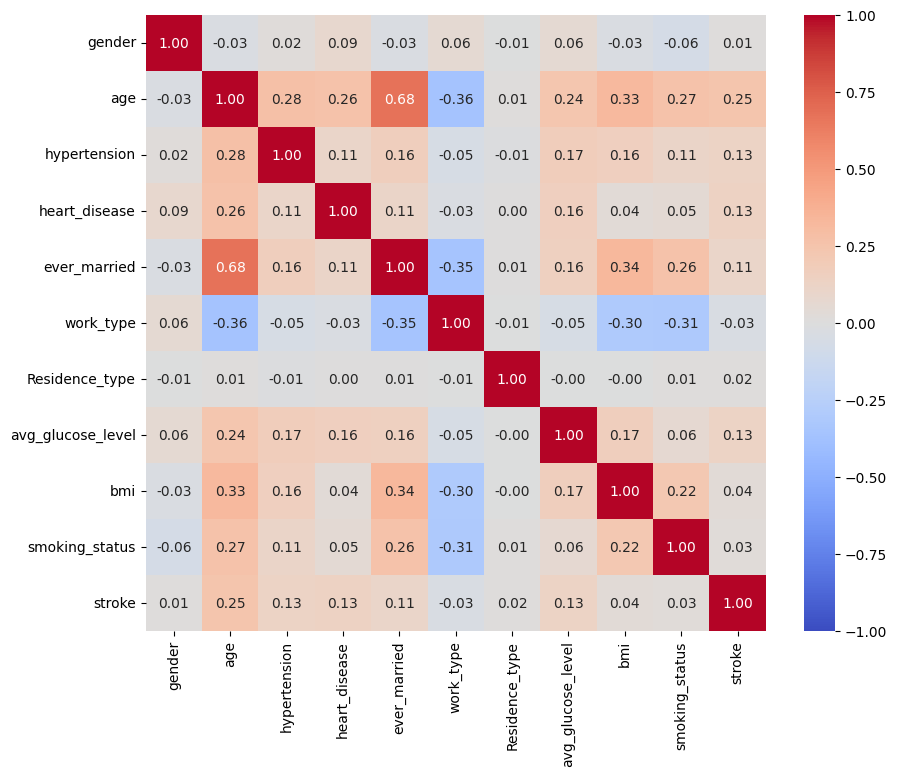
\includegraphics[width=0.64\textwidth]{CorrelationPlot.png}
\caption{Correlation between age and all other attributes except gender and residence type.}
\end{figure}


The histograms provide more information about multi-categorical variables. People with “Self-employed worktype”, represented by a 3 on the histogram, have a higher proportion of people who had a stroke. Children are, as expected, very unlikely to have a stroke. However, the histogram of “smoking\_status” is strange. The “formerly smoked” people counter-intuitively have a higher proportion of people with strokes than the “smokes” people, and people with “Unknown” status have a lower proportion of people who had a stroke than even the group that never smoked. This observation supports that one-hot encoding of “work type” and “smoke status” is crucial, and opposes the idea of replacing “unknown” with “smoke”. 
Based on the above observation, we can predict that the model will have the highest weight on “age”.

\begin{figure}[ht]
\centering
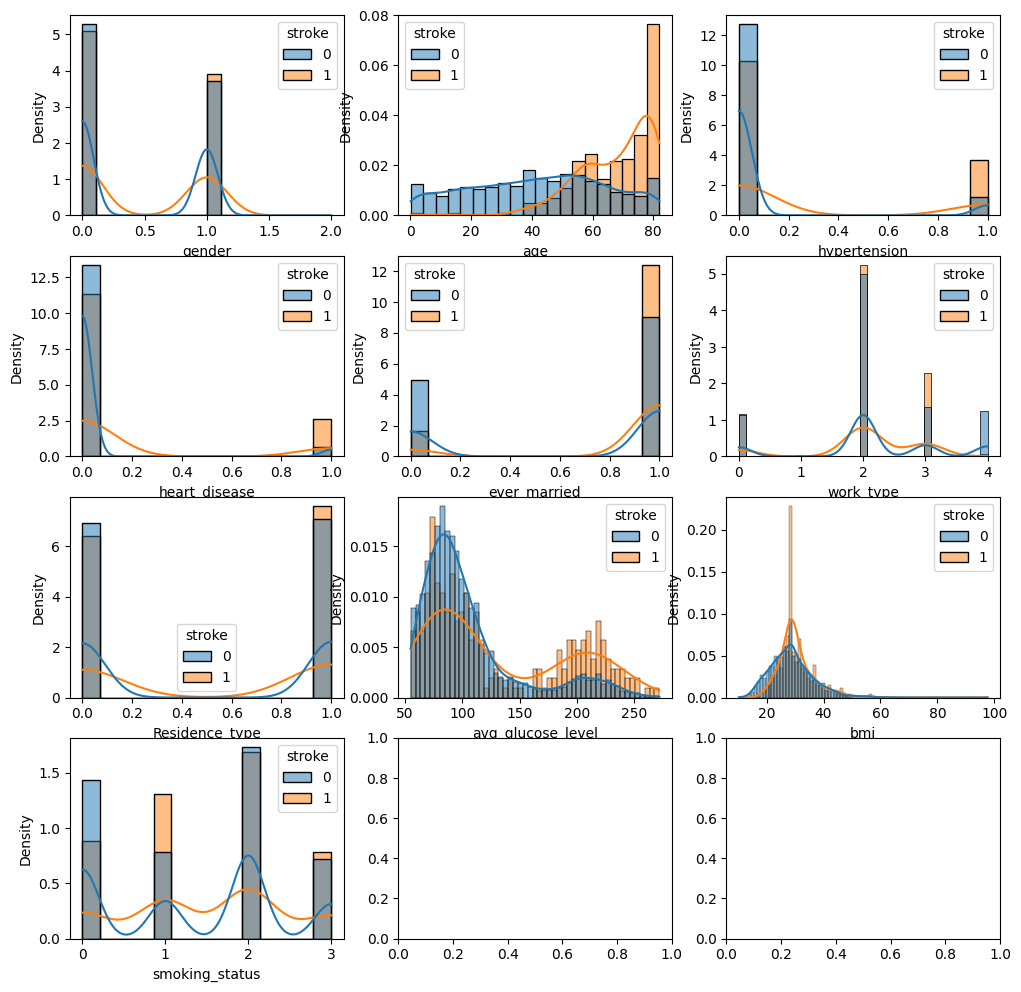
\includegraphics[width=0.7\textwidth]{Density.png}
\caption{Strong predictors of stroke include age, heart\_disease, hypertension, avg\_gluclose\_level.}
\end{figure}

For each of the categorical attributes, we encode the set of categories in the following way:
\begin{description}
    \item[gender] \{`Female': 0, `Male': 1, `Other': 2\}
    \item[ever\_married] \{`No': 0, `Yes': 1\}
    \item[work\_type] \{`Govt\_job': 0, `Never\_worked': 1, `Private': 2, `Self-employed': 3, `children': 4\}
    \item[Residence\_type] \{`Rural': 0, `Urban': 1\}
    \item[smoking\_status] \{`Unknown': 0, `formerly smoked': 1, `never smoked': 2, `smokes': 3\}
\end{description}
For attributes ``work\_type'', ``Residence\_type'', apply one-hot encoding.

\section*{Experimental Results}

When building the model, we use GridSearch to optimize the hyper-parameters of each model (when needed) and use cross-validation to check the accuracy and recall of each model. Recall for stroke is an important metric to predict true positives on stroke patients. This is something we are looking for in our models since we want to correctly predict a patient's risk for stroke rather than not, which can potentially be life threatening. Precision for stroke will be low across our models as expected, given that we did not oversample the testing data to validate our results.

\medskip

\textbf{Optimal Hyperparameters}

Neural Network: \texttt{\{`hidden\_layer\_sizes': (15, 10)\}} \\
Naive Bayes Classifier: \texttt{\{`var\_smoothing': 0.001\}} \\
SVM Classifier: \texttt{\{`C': 100, `gamma': 1, `kernel': `rbf'\}} \\
Random Forest: \texttt{\{`max\_depth': 10, `n\_estimators': 14\}} \\
K Nearest Neighbors: \texttt{\{`metric': `manhattan', `n\_neighbors': 3, `weights': `distance'\}}

\begin{figure}[ht]
\centering
\includegraphics[width=1\textwidth]{table.png}
\caption{Random Forest model achieved the best outcome, at 88\% test accuracy. With the Stacking Classifier, we were able to achieve the highest test accuracy of 90\%. Logistic Regression (73\% Recall), Multi-layer Perceptron (87\% Recall),  Gaussian Naive Bayes (85\% Recall) would work best for predicting stroke risk patients.}
\end{figure}

\begin{figure}[ht]
\centering
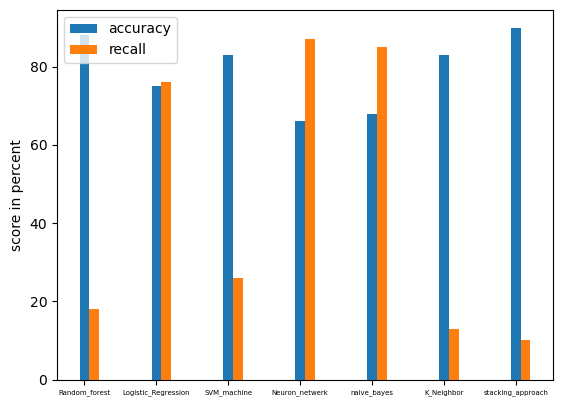
\includegraphics[width=0.55\textwidth]{Models.png}
\caption{Logistic Regression strikes a good balance between 76\% accuracy and 75\% recall.}
\end{figure}

\section*{Conclusion}

Synthetic Minority Oversampling Technique (SMOTE) was effective in improving the models’ precision/recall for stroke patients. Our initial hypothesis proved to be correct. Random Forest produced the best accuracy. By applying multiple algorithms using a stacking approach, we were able to achieve an even higher accuracy than the Random Forest model. However, both the recall scores are much lower than we had hoped. Further study is needed to determine the reason, however, one hypothesis is that the lower recall models feeding into it are the likely culprit. In this case, an interesting trial to attempt in the future would be to apply the stacking classifier strategy to only high recall algorithms and see how it performs.

\medskip

Despite the lower accuracy, models like Logistic Regression, Multi-layer Perceptron, and Naive Bayes would work better in predicting stroke risk patients given its high recall.
Logistic Regression is the most comprehensive model given its good balance between accuracy and recall, which was also the most consistent in predicting stroke patients through our web based front-end. As a result, this is the most comprehensive model that we have decided on.

\medskip

By checking the weight/importance of each attribute, we can determine that no matter which model we look at, the “age” variable always has the highest influence on classification. This maps well with our findings during data exploration.

\medskip

When testing the model on a test dataset without oversampling, it’s obvious that our model is more accurate at recognizing healthy people with no stroke. However, it is much less accurate when attempting to indicate people at risk of a stroke.  We believe that this discrepancy is caused by the low natural probability of having a stroke and the idea that the in-risk category is much broader than the has had a stroke category.

\medskip

Finally, reflecting on our results and process indicates that a future study should focus on  better optimization of hyper-parameters, and try to apply some more advanced strategies to the current model, such as Dropout regularization in neural networks. Additionally, changing up the algorithms included in the stack may generate very different results and due to its promise as a method, this is an opportunity well worth exploring.

\newpage
\begin{thebibliography}{99}
\bibitem{dritsas2022} 
Dritsas, Elias, and Maria Trigka. ``Stroke Risk Prediction with Machine Learning Techniques.'' \emph{Sensors}, vol. 22, no. 13, 21 June 2022, p. 4670. \url{https://doi.org/10.3390/s22134670}.

\bibitem{fedesoriano2021}
Fedesoriano. ``Stroke prediction dataset.'' Kaggle, 26 January 2021. \url{https://www.kaggle.com/datasets/fedesoriano/stroke-prediction-dataset}.

\bibitem{mainali2021} 
Mainali, Shraddha, et al. ``Machine Learning in Action: Stroke Diagnosis and Outcome Prediction.'' \emph{Frontiers in Neurology}, vol. 12, 6 Dec. 2021. \url{https://doi.org/10.3389/fneur.2021.734345}.

\bibitem{tazin2021} 
Tazin, Tahia, et al. ``Stroke Disease Detection and Prediction Using Robust Learning Approaches.'' \emph{Journal of Healthcare Engineering}, vol. 2021, 26 Nov. 2021, p. e7633381. \url{https://doi.org/10.1155/2021/7633381}.
\end{thebibliography}

\newpage
\section*{Project Roadmap}

\subsection*{Week 3 - Describing the problem scientifically}
For this week, our focus is to find a suitable dataset and topic for the project. We will prepare a 1 page write up, describing the problem scientifically and explaining the goal of the project along with deliverables. Following this, we will consult with the professor to validate our project topic.

\subsection*{Week 4 - Background Study}
During this week, we will conduct an in-depth literature review on stroke prediction research. The key is to gather information and understand existing findings about stroke prediction. This is essential to identify gaps in previous studies and how our project might fill them. We will complete the introduction and literature review for our project report.  

\subsection*{Week 5 - Dataset: Understanding and Exploratory Data Analysis}
This week is dedicated to exploratory data analysis and writing up our dataset description. We’ll familiarize ourselves with our dataset, understanding its structure and plans to build a machine learning model. We’ll analyze our dataset to uncover trends, correlations, and potential issues with the data.

\subsection*{Week 6 - Developing Accurate Prediction Model(s)}
This week, we aim to develop a comprehensive machine learning model of our dataset. We’ll experiment with different algorithms and techniques to find the most effective approach for stroke prediction. The model’s initial performance will be evaluated, and necessary adjustments will be made based on these results.  

\subsection*{Week 7 - Evaluation of the model(s) and Testing the performance}
This week, we will evaluate the performance of our final model in predicting stroke patients. We aim to continue to enhance its accuracy and reliability by fine tuning the parameters. In addition, we will finish up our project report by writing up the experimental results and conclusion.

\subsection*{Week 8 - Developing a basic web-based front-end }
This week, we will build a web based front-end for our machine learning model. This will allow users to invoke and run our model on input patient data and display the stroke prediction output.

\subsection*{Week 9 - Create and prepare for presentation}
This is the final week for wrapping up our project. We’ll finalize our model and web based front-end, ensuring that everything is tested and working properly. We will also prepare presentation slides based on our completed final report. 

\subsection*{Week 10 - Presentation}
This week, we will rehearse our presentation and deliver our findings to the class.

\end{document}